%!TEX program = xelatex
\documentclass[xcolor={table}]{beamer}

\usepackage[brazil]{babel}	
\usepackage[utf8]{inputenc}
\usepackage[T1]{fontenc}
\usepackage[scaled]{helvet}
\usepackage{amsthm}
\usepackage{ragged2e}
\usepackage{subfig}
\usepackage[table]{xcolor}
\usepackage{multicol}
\usepackage{multirow}
\usepackage{fancyvrb}
\usepackage{verbatim}

\usetheme{Execushares}

\title{Laborator 1 - \\
Sistemul de întreruperi}
\subtitle{}
\author{Coca Mihai \\
        Ioana Dragoș}

\setcounter{showSlideNumbers}{1}

\begin{document}
	\setcounter{showProgressBar}{0}
	\setcounter{showSlideNumbers}{0}

	\frame{\titlepage}

	\begin{frame}
		\frametitle{Tabelă de Conținut}
		\begin{enumerate}
			\item Concepte introductive
			\item Sistemul de întreruperi
		\end{enumerate}
	\end{frame}

	\setcounter{framenumber}{0}
	\setcounter{showProgressBar}{1}
	\setcounter{showSlideNumbers}{1}
	\section{Concepte introductive}
	\begin{frame}
		\frametitle{Noțiuni de bază}
        \begin{center}
        \begin{table}
        \begin{tabular}{ |c||c|c|  }
         \hline
         \multicolumn{3}{|c|}{\textbf{Microprocessor \textit{(single-chip CPU)} vs Microcontroller}} \\
         \hline
         \hline
         \textbf{Componentă}  &  \textbf{MPU} &  \textbf{MCU}\\
         \hline
         \textbf{Arhitectură}   & Von Neumann   & Harvard\\
         \hline
         \textbf{Memorie \& I/O} &   Externe (c.extinse)  & Interne (c. compacte)\\
         \hline
         \textbf{CLK} & Frecvențe mari (\sim GHz) & Frecvențe mici (\sim MHz)\\
         \hline
         \textbf{Consum}    & Mare & Mic\\
         \hline
         \textbf{Instrucțiuni} &   Operații externe & Operații interne\\
         \hline
         \textbf{Programe} & Complexe  & Simpliste și specializate\\
         \hline
         \textbf{SO} & Suportă ( >1GHz)  & RTOS(deterministic)\\
         \hline
        \end{tabular}
        \caption{\label{tab:1} Diferențele între microprocesor și microcontroller}
        \end{table}
        \end{center}
	\end{frame}

		\begin{frame}
			\frametitle{Sistem embedded}
			\begin{itemize}
				\item Este un \textbf{\textit{sistem}} care utilizează unul sau mai multe microcalculatoare pentru a rula programe personalizate, dedicate și conectate la cel puțin o componentă hardware specializată, în scopul expunerii către utilizator a unui set dedicat de funcții
				\item PC-urile nu sunt proiectate în scopul rulării unui singur task dedicat unui set specializat de componente hardware
				\item \textbf{Exemple} - pilot automat masină, termostat AC, regulator semafor, controler sistem irigare, osciloscop, Mars Rover etc.
			\end{itemize}
		\end{frame}
		
		\begin{frame}{}
		    \frametitle{Microcontroller}
		    \begin{itemize}
		    \item \textbf{Microcontroller} - componentă single-chip care conține pe lângă MPU, memorii de tip ROM, RAM, periferice (GPIO), timere și canale de comunicație serială, toate în același chip (“most compact design and the lowest hardware cost”)
		    \item \textbf{Configurație} -  dimensiune CPU (8, 16 maxim 32 biți), frecvență CPU (ordin 100 MHz)
		    \end{itemize}
		    
		\end{frame}
		
		\begin{frame}{}
		    \frametitle{Embedded Programming}
		    \begin{itemize}
		    \item \textbf{\textit{Initializare}} -  startup code înainte de apelul main() \& user program
		    \item Un program creat pentru o platformă embedded va conține în general \textbf{\textit{manipulări de biți}}, atât pentru intrări cât și pentru ieșiri
            \item Un MCU va avea mulți regiștrii de \textbf{\textit{configurare}} și de \textbf{\textit{stare}} care sunt manipulați prin setarea, ștergerea, citirea unor biți individuali 
            \item Fiecare \textbf{\textit{registru}} poate fi găsit la o adresă fixă de memorie
		    \item \textbf{Cunoștiințe necesare} -  o bună înțelegere a echipamentelor de depanare, precum: multimetru, osciloscop, analizator logic etc.
		    \item `all microcontroller programming is embedded programming'
		    \end{itemize}
		    
		\end{frame}

	\section{Sistemul de întreruperi}
		\begin{frame}
			\frametitle{Întrerupere}
			\begin{itemize}
			    \item \textbf{\textit{Întrerupere}} - semnal transmis procesorului, emis fie de către un eveniment hardware/software, cu scopul execuției imediate (după terminarea instrucțiunii curente) a unei rutine de întreruperi
			    \item \textbf{\textit{ISR - Interrupt Service Routine }} reprezintă secvența de cod \textit{invizibilă} (este salvat contextul codului întrerupt, iar după execuția rutinei este refăcut)  executată ca răspuns la apariția unei anumite întreruperi
			    \item Întreruperile mascabile pot fi activate/dezactivate
			\end{itemize}
		\end{frame}

				\begin{frame}
			\frametitle{Tipuri de întreruperi}
			\begin{itemize}
			    \item \textbf{\textit{Hardware}} - asincrone, nu sunt relaționate de codul curent executat de procesor
			    \item \textbf{\textit{Software}} - sincrone, sub formă de excepții, reprezintă rezultatul unor instrucțiuni specifice
			\end{itemize}
		\end{frame}

		\begin{frame}
			\frametitle{NVIC}
			\begin{itemize}
		       \item \textbf{\textit{Nested Vectored Interrupt Controller}}
			\end{itemize}
    			 \begin{figure}
                \centering
               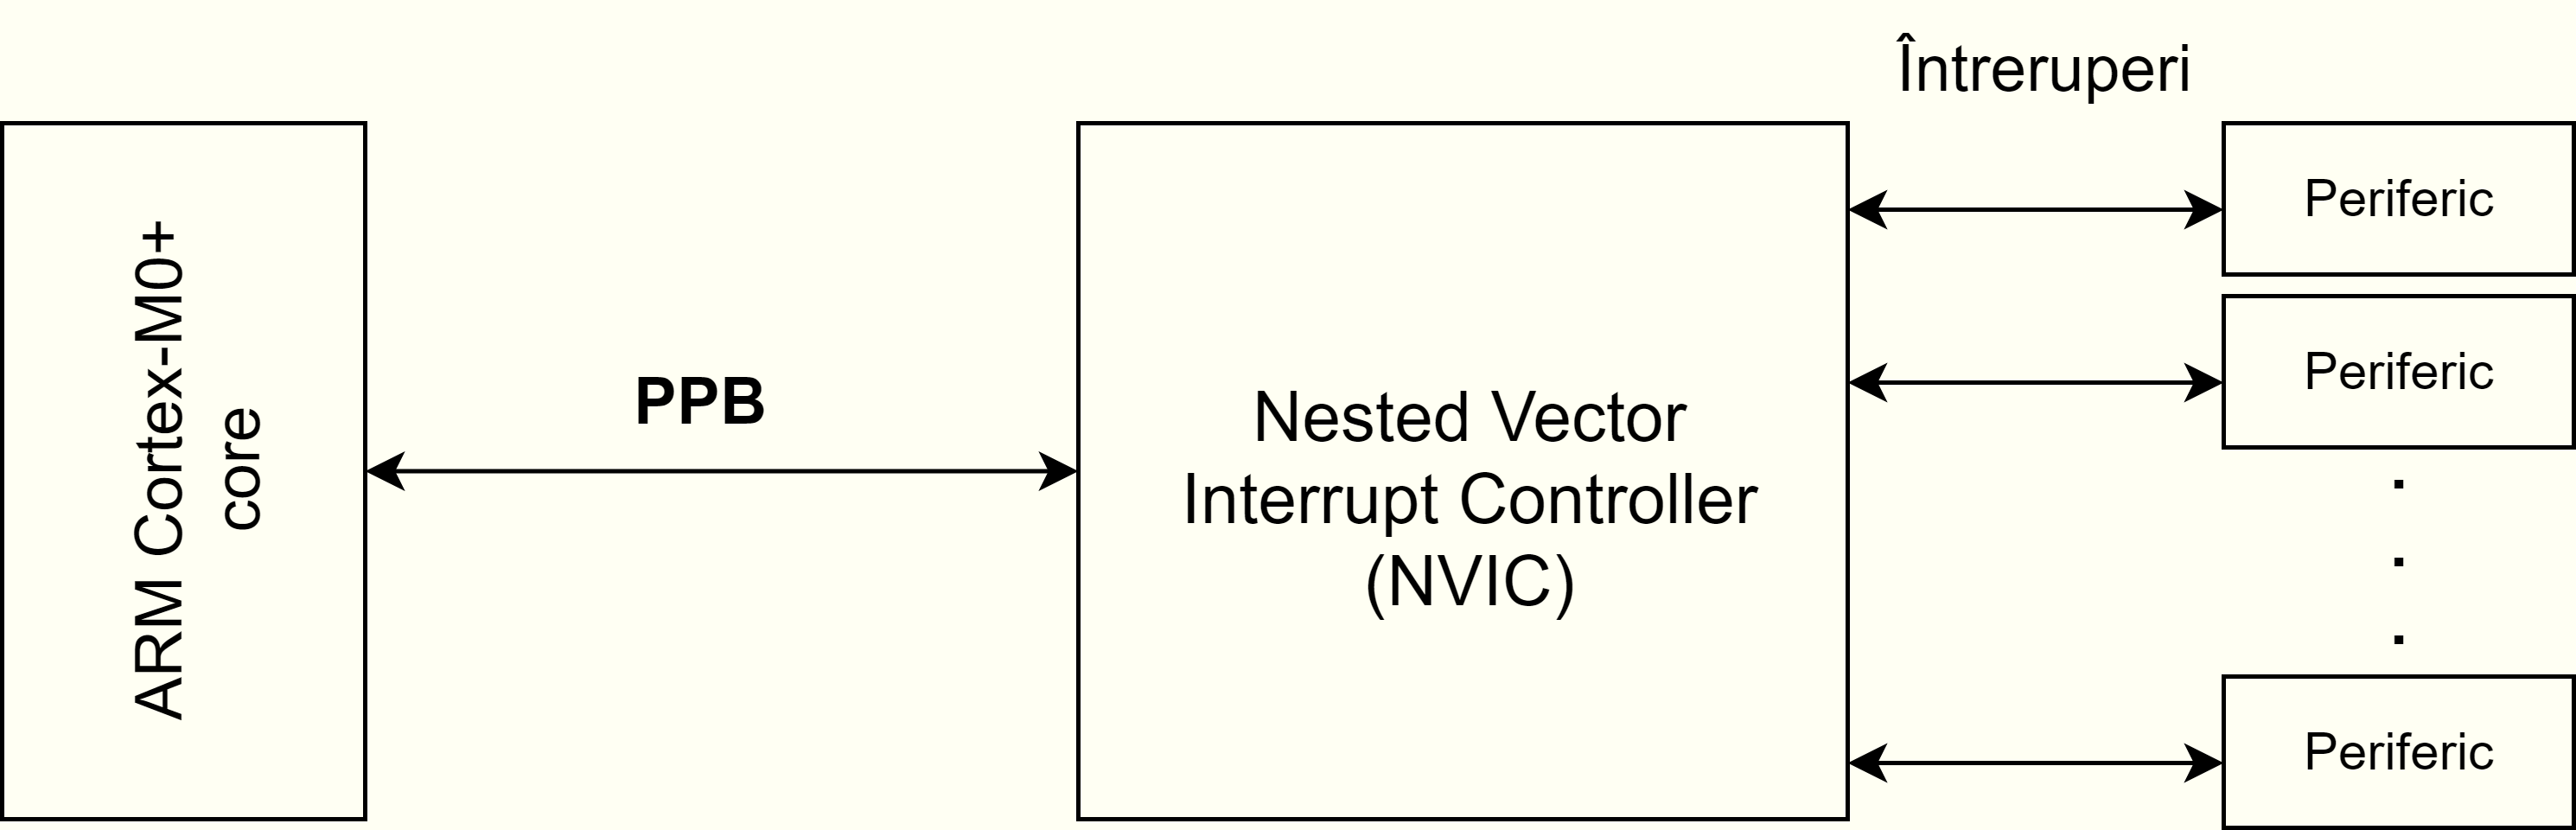
\includegraphics[width=9.5cm]{images/nvic.png}
            \end{figure}
            \begin{itemize}
		       \item Reprezintă o \textit{tabelă} (vector) a adreselor rutinelor de tratare a întreruperilor (\textit{ISR}) împreună cu numărul asociat și are rolul de a manageria și prioritiza întreruperile externe 
			\end{itemize}
		\end{frame}
		
				\begin{frame}
			\frametitle{NVIC}
			\begin{itemize}
		       \item Execuția codului curent este suspendată
		       \item Contextul programului este salvat
		       \item NVIC inițiază un apel către vectorul de adrese, localizează numărul întreruperii care a avut loc, extrage adresa rutinei de întreruperi
		       \item Secvența de cod asociată rutinei este executată
		       \item Contextul este readus și execuția programului este reluată
			\end{itemize}
		\end{frame}
		\begin{frame}
		    \frametitle{Sistemul de întreruperi}
		    \begin{itemize}
		        \item Un MCU este proiectat în general pentru a răspunde la un număr de surse diferite de întrerupere (10 – 100 de surse). Fiecare sursă poate avea un cod specific scris de programator care este executat atunci când o întrerupere este desclanșată 
		        \item Programatorul decide care întreruperi vor fi active, precum și timpul de activare/dezactivare al acestora în execuția programului
		        \item \textbf{startup\_MKL25Z4.s} - conține tabela vectorilor de întreruperi, având 32 de handlere pentru întreruperi externe
		    \end{itemize}
		    
		\end{frame}
		
		\begin{frame}
            \frametitle{Sistemul de întreruperi}
            \begin{figure}
                \centering
                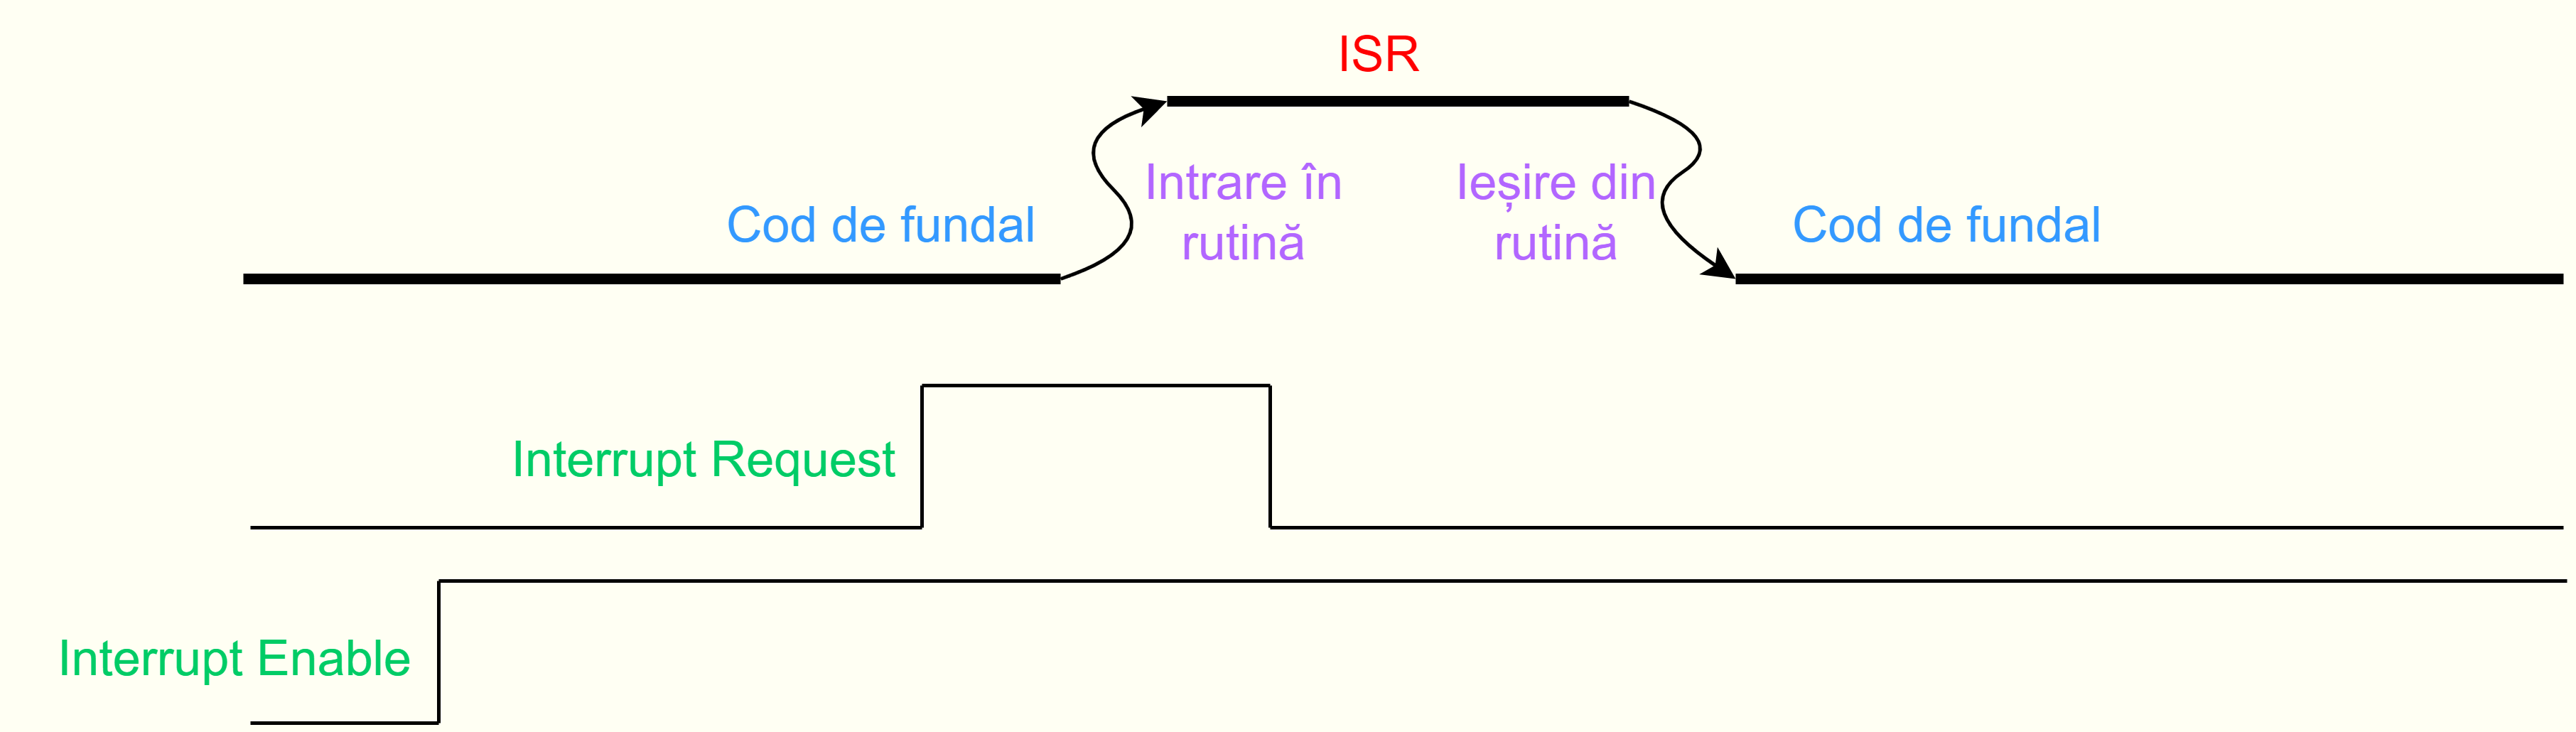
\includegraphics[width=9cm]{images/isr1.png}
                \caption{Întreruperea codului executat la apariția unei întreruperi}
            \end{figure}
            \begin{itemize}
                \item TVI va conține adresele de start a ISR-urilor asociate. Pentru întreruperile care nu vor fi active, intrările echivalente pot fi lăsate necompletate sau să pointeze către un ISR fictiv/default
                \item O funcție ISR trebuie să facă cât mai puțin posibil (menținerea unei latențe cât mai mici într-un sistem cu multiple surse de întrerupere active)

            \end{itemize}   
        \end{frame}
		\begin{frame}
            \frametitle{Sistemul de întreruperi}
            \begin{itemize}
                \item În mod normal, o cerere de întrerupere este salvată (\textit{latched}), ceea ce înseamnă că evenimentul de întrerupere setează un flag, a cărui stare persistă chiar dacă evenimentul este încheiat
            \end{itemize}
            \begin{figure}
                \centering
                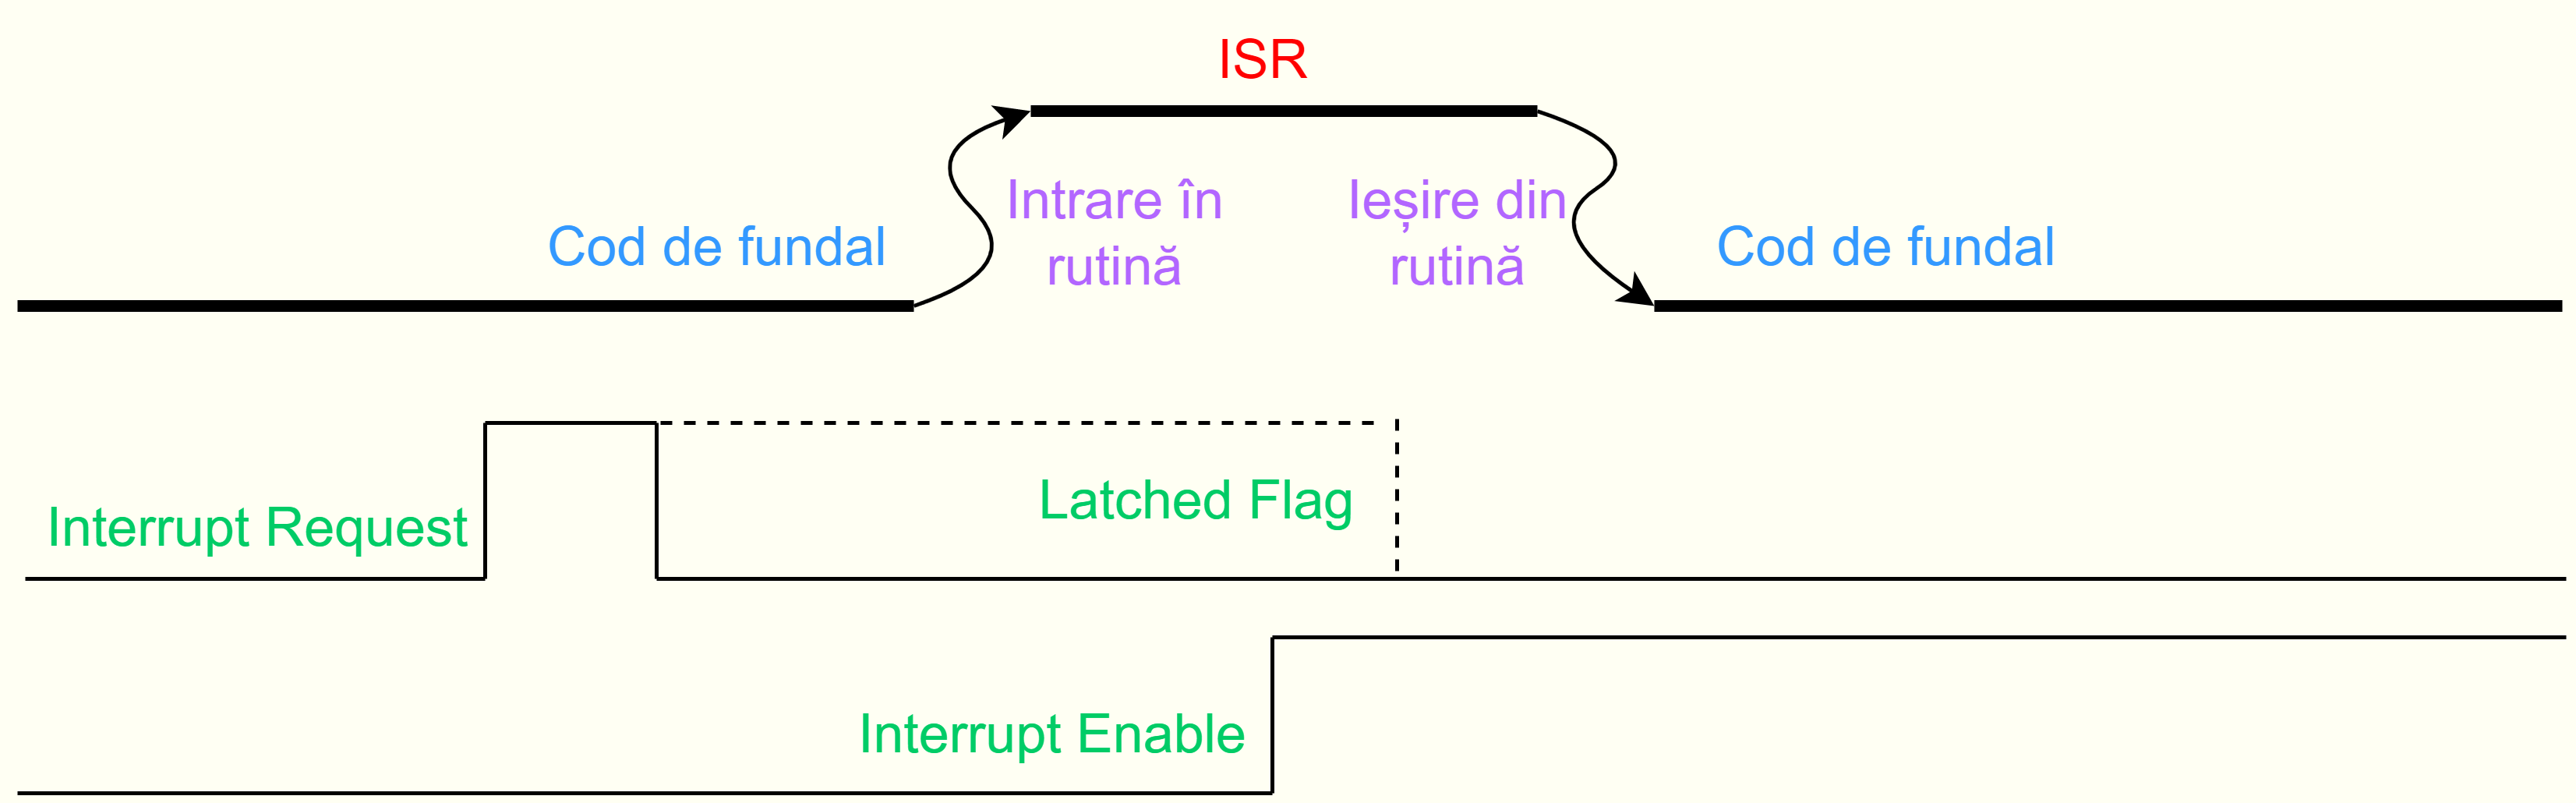
\includegraphics[width=9cm]{images/isr2.png}
            \end{figure}
		\end{frame}

		\begin{frame}
			\frametitle{Întreruperi multiple}
			\begin{itemize}
				\item Într-un sistem cu multiple surse de întrerupere active, pot să apară situații de concurență asupra execuției ISR-ului asociat (\textbf{\textit{scenariu}}: INT1 ISR se află în execuție  și apare o cerere de întrerupere INT2)
				\begin{enumerate}
				    \item INT2 este blocată până când INT1 ISR se execută integral
				    \item INT2 este mai prioritară decât INT1, iar INT1 ISR va fi întrerupt (se consideră faptul că INT2 va fi activată in interiorul INT1 din moment ce la intrarea într-un ISR, există o dezactivare globală a tuturor întreruperilor din sistemul respectiv)
				\end{enumerate}
			\end{itemize}
		\end{frame}
		\begin{frame}
		    \frametitle{Întreruperi multiple}
		    \begin{figure}
		        \centering
		        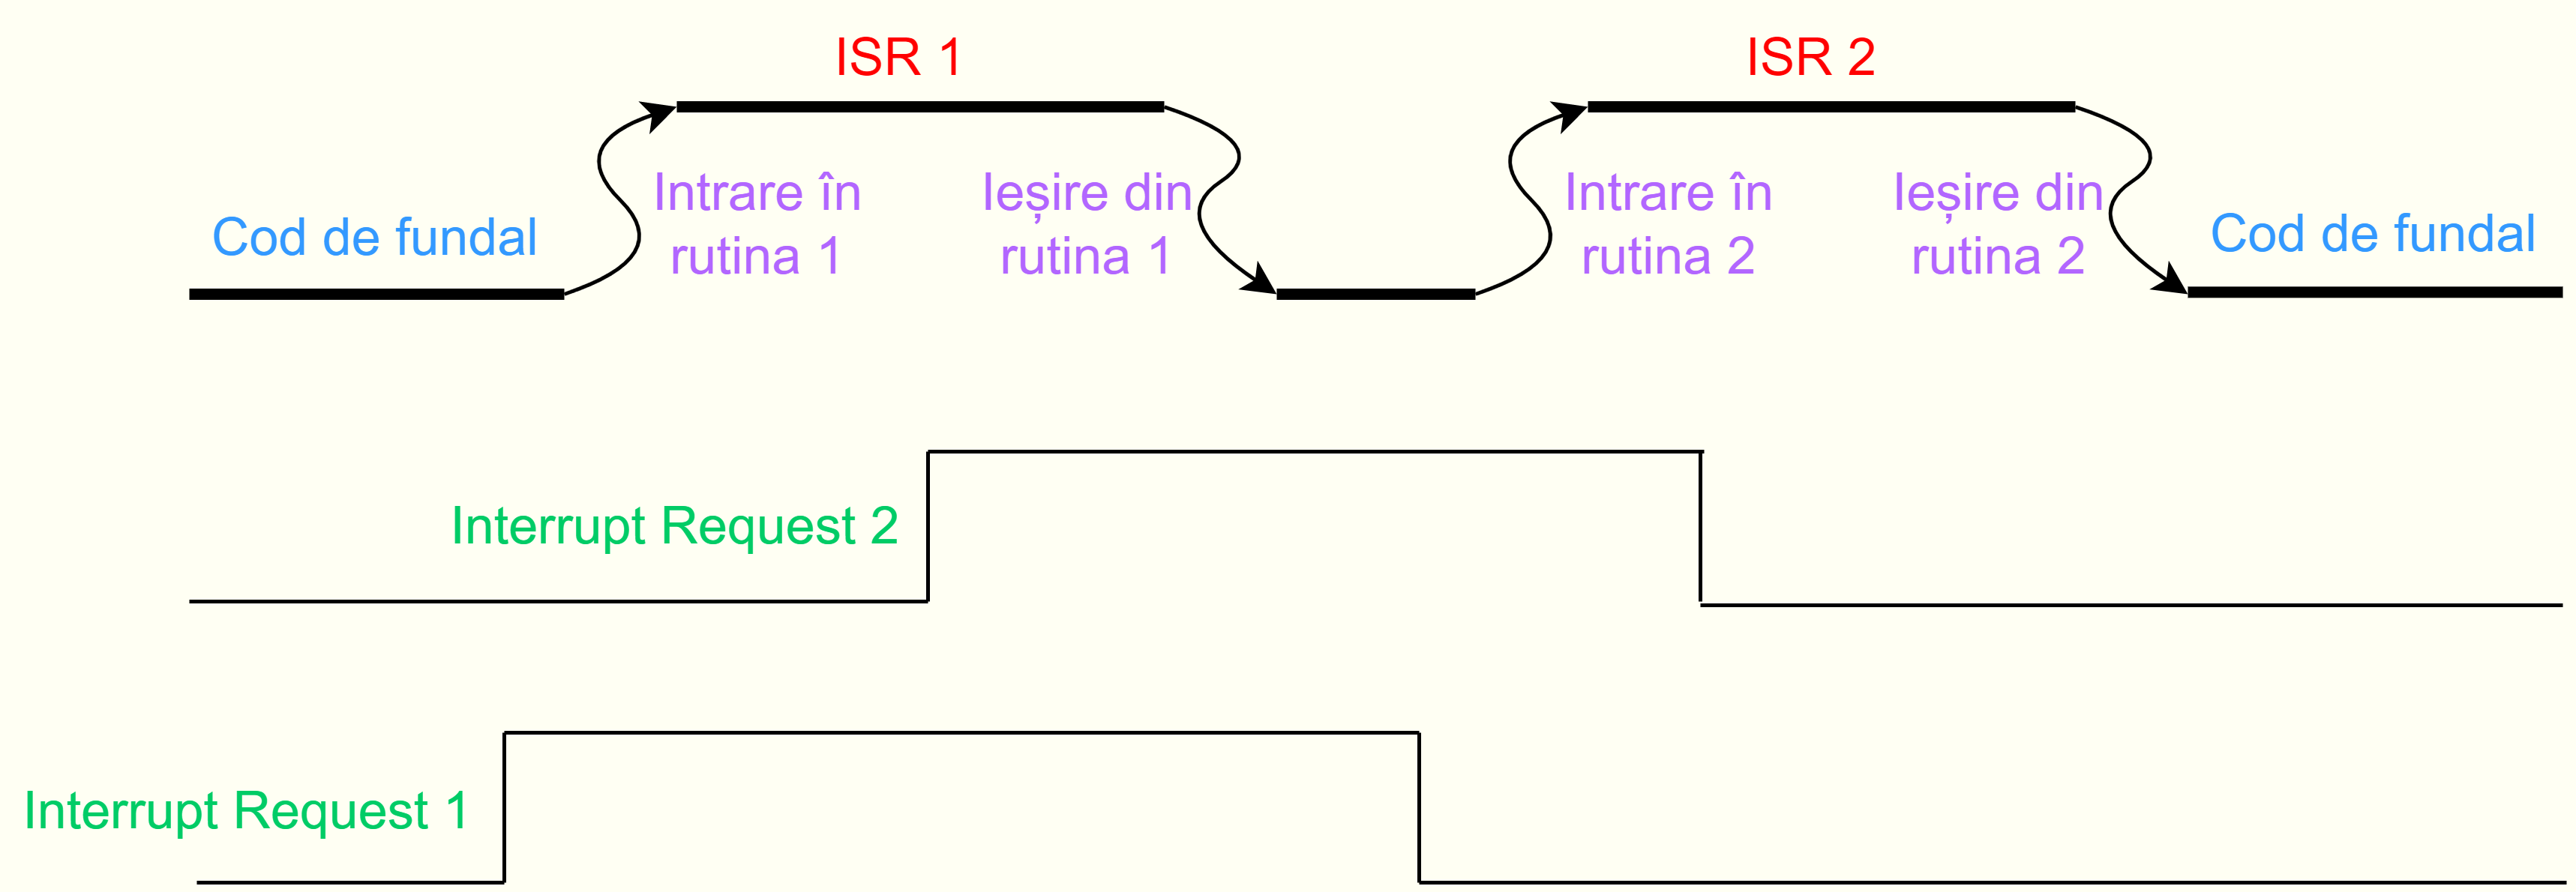
\includegraphics[width=8cm]{images/isr3.png}
		    \end{figure}
		    \hline
		    \begin{figure}
		        \centering
		        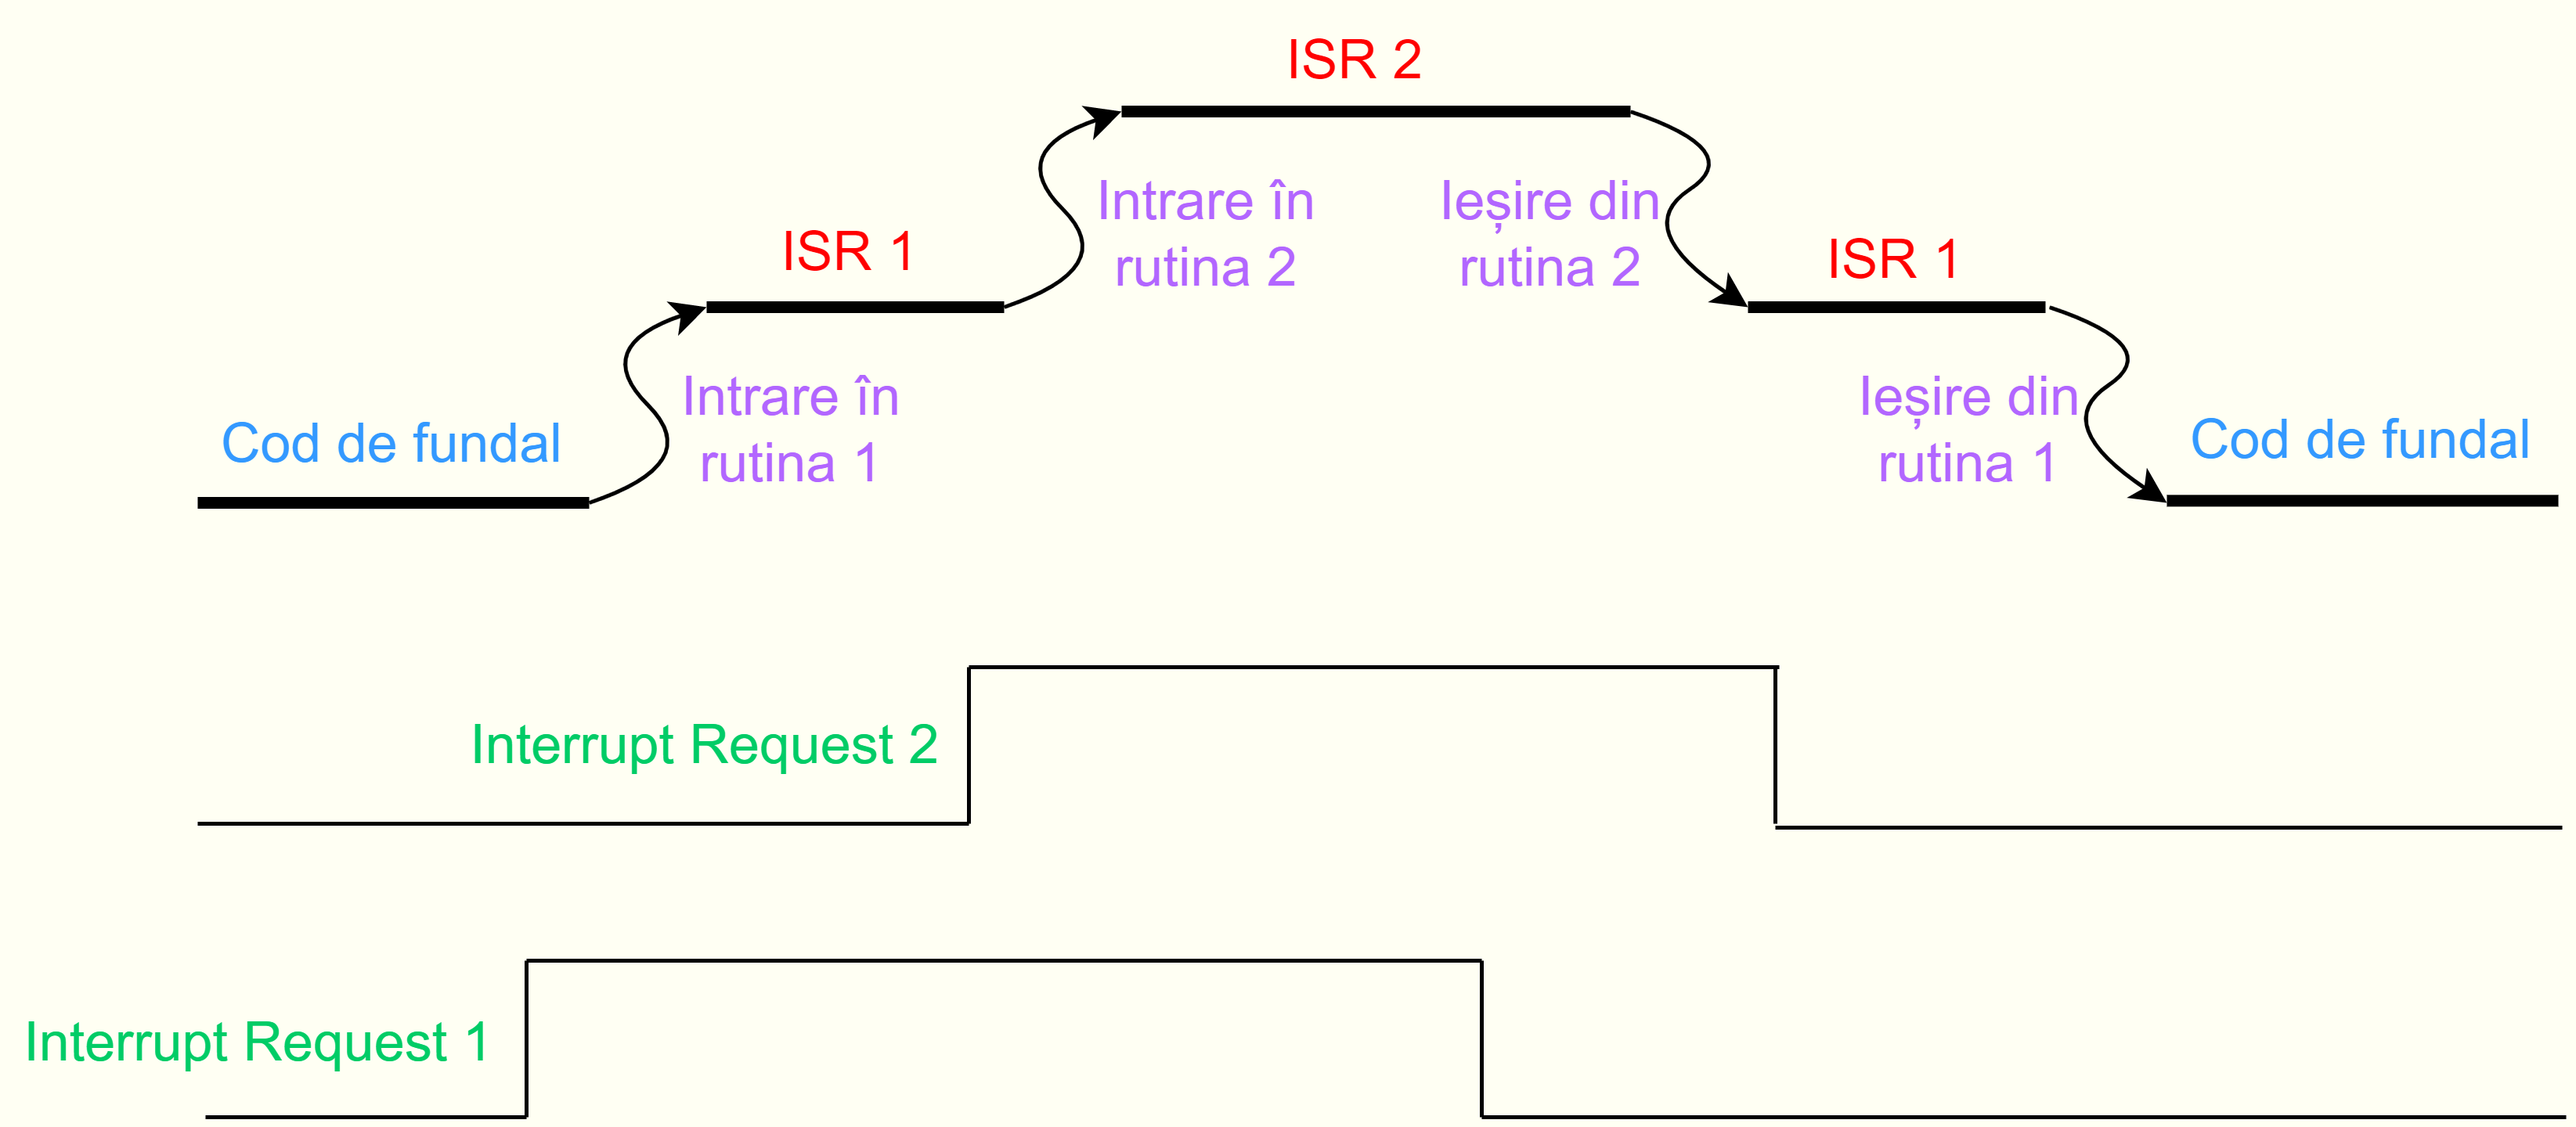
\includegraphics[width=8cm]{images/isr4.png}
		    \end{figure}
		\end{frame}
    	\begin{frame}
    	    \frametitle{Sistemul de întreruperi}
    	    \begin{itemize}
    	        \item Marcarea secțiunilor critice într-un scenariu de suprapunere a accesului la o zonă de memorie partajată (acces neîntrerupt la date prin dezactivarea întreruperilor cu acces la zona respectivă)
    	        \item În funcție de compilator, dacă o variabilă este folosită atât în mainline code cât și într-o funcție ISR, variabila respectivă trebuie declarată \textbf{\textit{volatile}}. Altfel, componenta de optimizare a compilatorului va genera un output inconsistent
    	    \end{itemize}
    	 \end{frame}
    	 \begin{frame}
    	    \frametitle{Sistemul de întreruperi}
    	    \begin{itemize}
    	        \item \textbf{\textit{Scenariu}}: de obicei funcțiile ISR modifică variabile care sunt testate în mainline code. De exemplu, o întrerupere pe un port serial setează un flag global
    	    \end{itemize}
    	     \begin{figure}
		        \centering
		        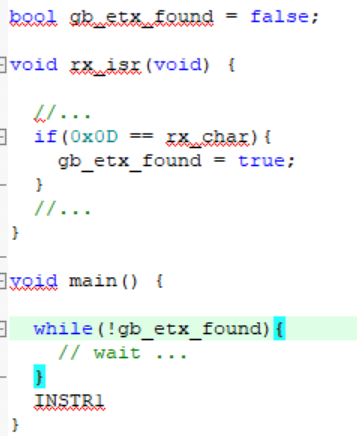
\includegraphics[width=4cm]{images/example-memory.png}
		    \end{figure}
    	 \end{frame}
    	 \begin{frame}
    	    \frametitle{Sistemul de întreruperi}
    	    \begin{itemize}
    	        \item Compilatorul nu știe că variabila \textit{gb\_etx\_found} ar putea fi modificată în ISR din moment ce nu apare niciun apel către ISR. Compilatorul observă că expresia \textit{\textbf{!gb\_ext\_found}} va fi întotdeauna true, rezultând într-o buclă infinită, eliminând astfel din executabilul final INSTR1 (unreachable code)
    	    \end{itemize}
    	 \end{frame}
    	 \begin{frame}
    	    \frametitle{Sistemul de întreruperi}
    	    \centering
    	    \begin{itemize}
    	        \item \textbf{\textit{Edge-triggered}} - dacă apăsăm o tastă din tastatura telefonului pentru mai multe secunde, un singur caracter va fi inserat (o acțiune este efectuată doar dacă semnalul suferă o tranziție $\textbf{0} \rightarrow \textbf{1}, \textbf{1} \rightarrow \textbf{0}$) 
    	        \item \textbf{\textit{Level-triggered}} - dacă apăsăm o tastă din tastatura PC-ului pentru mai multe secunde, vom obține un string de caractere (o acțiune este efectuată atât timp cât un semnal este activ în funcție de polaritate, \textbf{0} sau \textbf{1})
    	    \end{itemize}
    	     \begin{figure}
		        \centering
		    \end{figure}
    	 \end{frame}
	\appendix


\end{document}